%----------------------------------------------------------------
%
%  File    :  survey-browsers.tex
%
%  Author  :  Keith Andrews, IICM, TU Graz, Austria
%
%  Created :  27 May 1993
%
%  Changed :  16 Nov 2010
%
%----------------------------------------------------------------


\chapter{HTML Tables}

\label{HTML5 Tables}

In case of having too much data to display, or data which is inherently better in a grid, HTML tables
are the best solution available. Before, tables have been used mostly for the layout of
HTML websites (and is now an example of bad website development pracices) mainly due to two reasons:
\begin{itemize}
    \item[--] Semantically, it is wrong.
    \item[--] Tables aren't as adaptable and flexible as divs'
\end{itemize}

\section{Structure of Tables}

The basic structure of an HTML table starts with the \textit{<table>} tag. It is the starting
point for constructing a table. Now, HTML tables consist of columns and rows, like normal
tables. For rows, the tag  \textit{<tr>} is used, whereas for table header \textit{<th>} tag
is used. Normally, table headers are positioned in the center and are bold. For table cells
\textit{<td>} tag is used \parencite{7}.
\newpage

\begin{lstlisting}[%
    language = HTML,
    xleftmargin=0cm,              % no extra margins for floats
    xrightmargin=0cm,             % no extra margins for floats
    language=biblatex,
    basicstyle=\footnotesize\ttfamily,
    frame=shadowbox,
    numbers=left,
    label=list:BibACMIEEE,
    ,
]
    % An example of an HTML Table which demonstrates information about cars:
    <!DOCTYPE html>
<html>
<head>
	<title>Best Cars 2019</title>
</head>
<body>
<table class="table table-bordered table-hover table-condensed">
	<thead>
		<tr>
			<th title="Field #1">Car</th>
			<th title="Field #2">Manufacturer</th>
			<th title="Field #3">Engine Size</th>
			<th title="Field #4">Cylinders</th>
			<th title="Field #5">Horsepower</th>
			<th title="Field #6">Torque</th>
			<th title="Field #7">Compresion Ratio</th>
			<th title="Field #8">Miles per gallon</th>
			<th title="Field #9">Price</th>
		</tr>
	</thead>
	<tbody>
		<tr>
			<td>2019 Acura RDX</td>
			<td>Acura</td>
			<td>2.00L</td>
			<td align="right">4</td>
			<td align="right">272</td>
			<td align="right">280</td>
			<td>9.8:1</td>
			<td align="right">28</td>
			<td>€33,600.00</td>
		</tr>
		<tr>
			<td>2019 Ford Ranger</td>
			<td>Ford</td>
			<td>2.30L</td>
			<td align="right">4</td>
			<td align="right">270</td>
			<td align="right">310</td>
			<td>10.0:1</td>
			<td align="right">21</td>
			<td>€21,800.00</td>
		</tr>
	</tbody>
</table>

</body>
</html>

\end{lstlisting}

Now, there exist more tags which can be used for HTML5 tables:
\begin{itemize}
    \item[--] $<$\texttt{thead}$>$ - Table header, it is used to point out single or multiple rows
of a table, which do not contain table data but column labels \parencite{8}.

    \item[--] $<$\texttt{tbody}$>$ - Table body, it is used to point out $<$\texttt{tr}$>$ elements. Position this tag
always after $<$\texttt{thead}$>$, but it can also come after or before $<$\texttt{tfoot}$>$ \parencite{8}.

    \item[--] $<$\texttt{tfoot}$>$ - Table footer, it is used to point out single or multiple $<$\texttt{tr}$>$ elements
where those elements are presenting an overview  of the data in the table \parencite{8}.

    \item[--] $<$\texttt{caption}$>$ - Table caption, as the name already says, can be used to specify table caption.
Can be put on the bottom of the CSS document.

    \item[--] $<$\texttt{col}$>$ - While using col and some other keyword, for example, align, it is possible direct
the alignment of text in the table. There are other keywords whom can be used to adjust colors, width
and many other things of table columns.
\end{itemize}




\chapter{Good Table Design}
We will discuss certain conventions that are widely regarded as ``Good Table Design''. These conventions are generally neat little CSS tricks which serve to aesthetically improve the look of a table and in most cases also add to the effectiveness and efficiency of tables. All tables must incorporate at least one of the following conventions.


\section{Alternate row highlighting}
When presented a table with a lot of entries, it can be hard to look at. Scrolling through numerous rows can be frustrating.
With this CSS trick, it can be a bit easier, at least for the eyes, if nothing else. The idea is to color every even row, while leaving
the odd ones intact.
Implementing this techniques requires only two lines of CSS, and is objectively useful.


\begin{lstlisting}[%
    language = HTML,
    xleftmargin=0cm,              % no extra margins for floats
    xrightmargin=0cm,             % no extra margins for floats
    language=biblatex,
    basicstyle=\footnotesize\ttfamily,
    frame=shadowbox,
    numbers=left,
    label=list:BibACMIEEE,
     stringstyle=\color{blue}
    ,
]
    % An example of using simple CSS to color table rows:

	table.alt tr:nth-child(even) {background: #CCC}
	table.alt tr:nth-child(odd) {background: #FFF}

\end{lstlisting}


An example HTML table with this technique is shown below.
\begin{figure}[H]
    \centering

    {%
    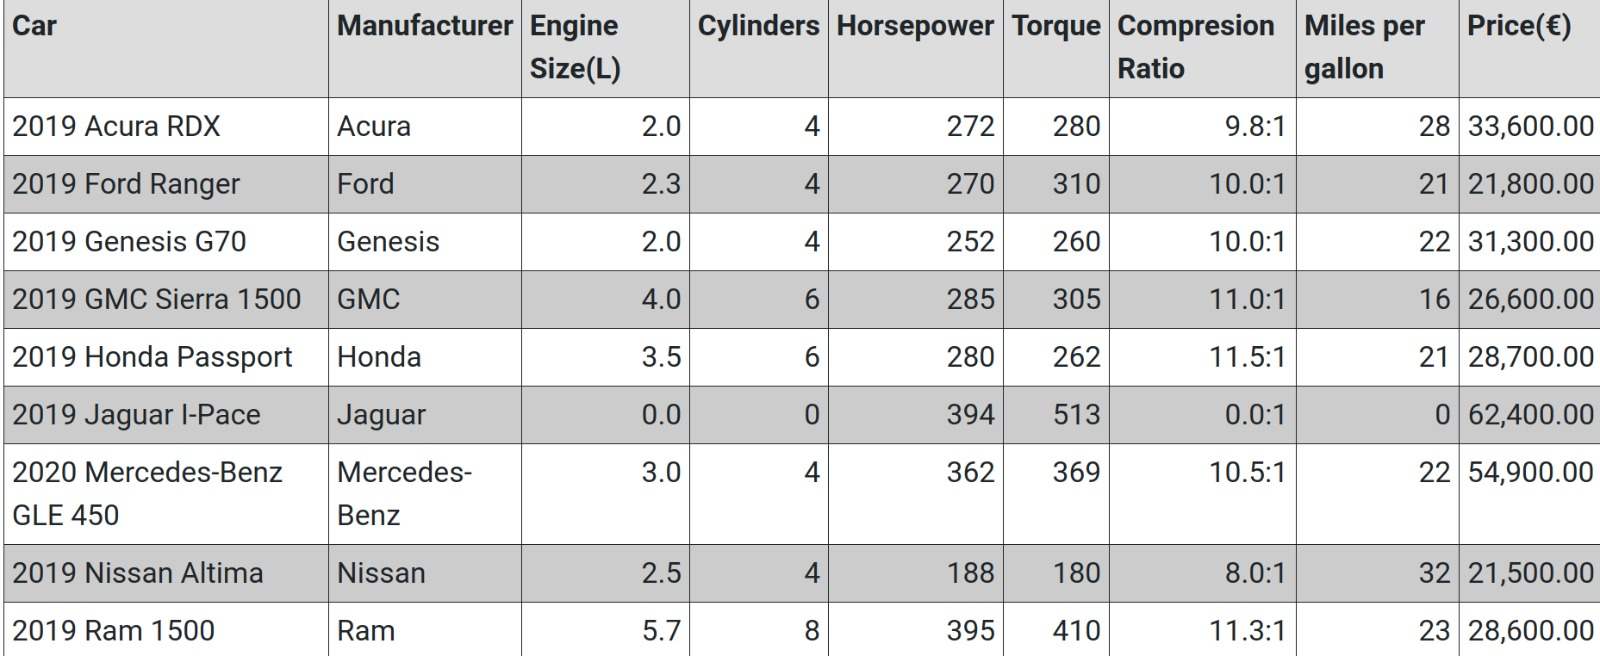
\includegraphics[width=\linewidth]
    {images/alt_t.jpeg}%
    \label{alig1}%
    }


    \caption[Alternate row highlighting]
    {

    \imgcredit{Screenshot taken by the author.}
    }
    \label{figAltRowHighlight}
\end{figure}


\newpage
\section{Current Row Highlighting}
Just like in Alternate Row Highlighting, `walking' through a big table one may
easily become lost and wouldn't know in which row he is at the moment, which can be
pretty stressful and overall decrease the efficiency of the table. 

With the help of some CSS, the lives of the users are made easier.

\begin{lstlisting}[%
    language = HTML,
    xleftmargin=0cm,              % no extra margins for floats
    xrightmargin=0cm,             % no extra margins for floats
    language=biblatex,
    basicstyle=\footnotesize\ttfamily,
    frame=shadowbox,
    numbers=left,
    label=list:BibACMIEEE,
     stringstyle=\color{blue}
    ,
]
    % An example of using simple CSS to highlight table rows:

	table {
      overflow: hidden;
	}

	tr:hover {
	  background-color: #ffa;
	}

	td, th {
	  position: relative;
	}
	td:hover::after,
	th:hover::after {
	  content: "";
	  position: absolute;
	  background-color: #ffa;
	  left: 0;
	  width: 100%;
	  z-index: -1;
	}

\end{lstlisting}


An example HTML table with this technique is shown below.
\begin{figure}[H]
    \centering

    {%
    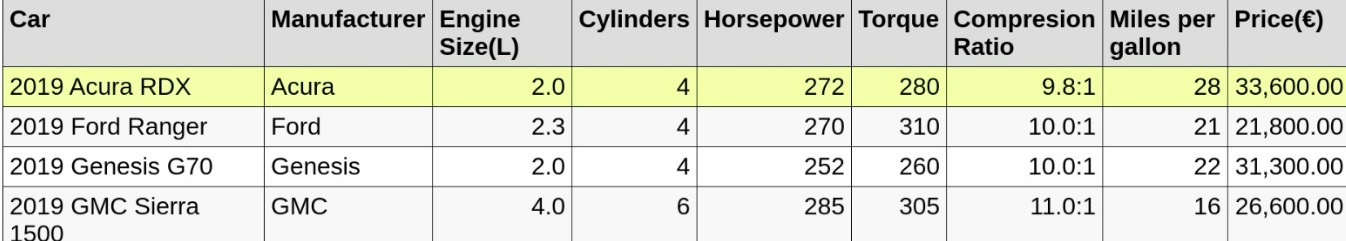
\includegraphics[width=\linewidth]
    {images/current_hl.jpeg}%
    \label{alig1}%
    }


    \caption[Current Row Highlighting]
    {

    \imgcredit{Screenshot taken by the author.}
    }
    \label{figCurrentRowHighlight}
\end{figure}

\section{Expandable Areas}
Should we have any further information available about a table's object,
making the row clickable and showing the extra information is a better
alternative than trying to cram everything inside the table. In the following code snippet
we see how additional data in an HTML table can be implemented. \parencite{10}

\begin{lstlisting}[%
    language = HTML,
    xleftmargin=0cm,              % no extra margins for floats
    xrightmargin=0cm,             % no extra margins for floats
    language=biblatex,
    basicstyle=\footnotesize\ttfamily,
    frame=shadowbox,
    numbers=left,
    label=list:BibACMIEEE,
     stringstyle=\color{blue}
    ,
]
<tr>
      <td>2019 Acura RDX</td>
      <td>Acura</td>
      <td style="text-align: right">2.0</td>
      <td style="text-align: right">4</td>
      <td style="text-align: right">272</td>
      <td style="text-align: right">280</td>
      <td style="text-align: right">9.8:1</td>
      <td style="text-align: right">28</td>
      <td style="text-align: right">33,600.00</td>
    </tr>
    <tr>
      <td colspan="5">
        <h4>Additional information about the car</h4>

        <ul>
          <li><a href="https://en.wikipedia.org/wiki/Acura_RDX">Acura RDX</a>
          </li>
          <li><a href="https://www.acura.ca/rdx">Acura RDX official webpage</a>
          </li>
        </ul>
      </td>
    </tr>
    <tr>
\end{lstlisting}
To implement this table feature the combination of JavaScript and
CSS needs to be implemented. In the snippet code below, the JavaScript and CSS code can be reviewed.

\begin{lstlisting}[%
    language = HTML,
    xleftmargin=0cm,              % no extra margins for floats
    xrightmargin=0cm,             % no extra margins for floats
    language=biblatex,
    basicstyle=\footnotesize\ttfamily,
    frame=shadowbox,
    numbers=left,
    label=list:BibACMIEEE,
     stringstyle=\color{blue}
    ,
]
<script type="text/javascript">
$(document).ready(function(){

  $("#report tr:odd").addClass("odd");
  $("#report tr:not(.odd)").hide();
  $("#report tr:first-child").show();

  $("#report tr.odd").click(function () {
    var trToToggle = $(this).next("tr");
    $("#report tr:not(.odd)").not(trToToggle).hide();
    $("#report tr:first-child").show();
    $(trToToggle).toggle();
    $(this).find(".arrow").toggleClass("up");
  });
})
</script>

\end{lstlisting}
\newpage

\begin{lstlisting}[%
    language = HTML,
    xleftmargin=0cm,              % no extra margins for floats
    xrightmargin=0cm,             % no extra margins for floats
    language=biblatex,
    basicstyle=\footnotesize\ttfamily,
    frame=shadowbox,
    numbers=left,
    label=list:BibACMIEEE,
     stringstyle=\color{blue}
    ,
]
#report {
    border-collapse:collapse;
}
#report h4 {
    margin:0px;
    padding:0px;
}
#report img {
    float:right;
}
#report ul {
    margin:10px 0 10px 40px;
    padding:0px;
}
#report th {
    background:#7CB8E2  repeat-x scroll center left;
    color:#fff;
    padding:7px 15px;
    text-align:left;
}
#report td {
    background:#C7DDEE none repeat-x scroll center left;
    color:#000;
    padding:7px 15px;
}
#report tr.odd td {
    cursor:pointer;
}
#report div.arrow {
    background:transparent url(arrows.png) no-repeat scroll 0px -16px;
    width:16px;
    height:16px;
    display:block;
}
#report div.up {
    background-position:0px 0px;
}
\end{lstlisting}

An example HTML table with this technique before a row is clicked is shown below.
\begin{figure}[H]
    \centering

    {%
    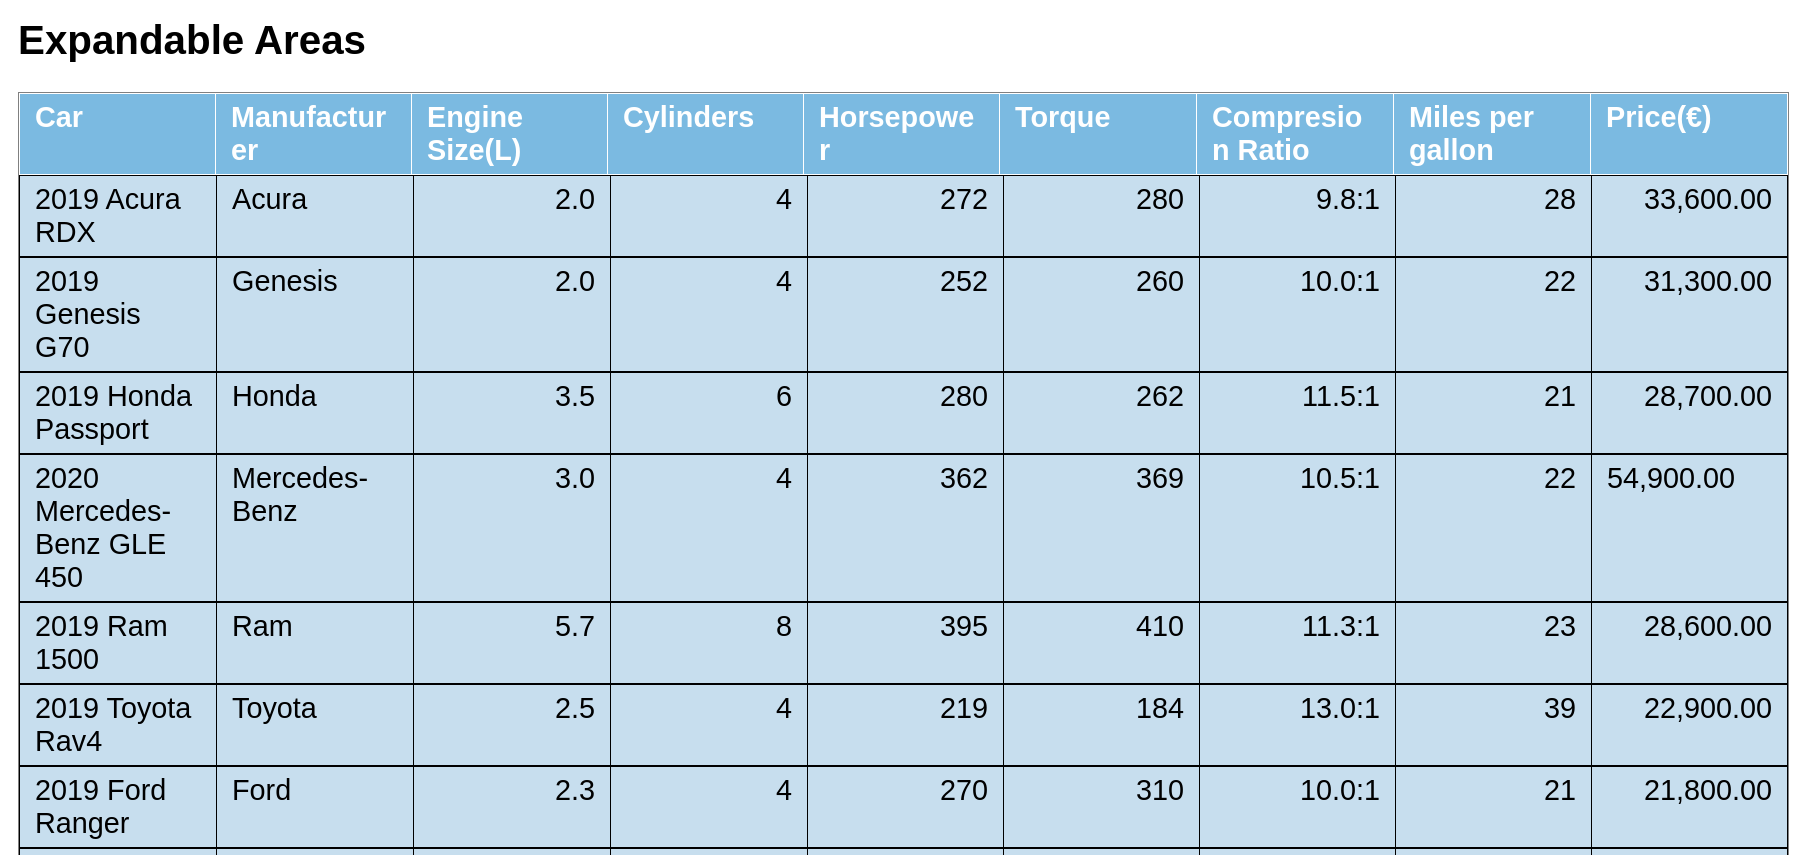
\includegraphics[width=\linewidth]
    {images/expandable_area_before.png}%
    \label{alig1}%
    }


    \caption[Expandable Areas]
    {

    \imgcredit{Screenshot taken by the author.}
    }
    \label{figExpandArea}
\end{figure}
An example HTML table with this technique after a row is clicked is shown below.
\begin{figure}[H]
    \centering

    {%
    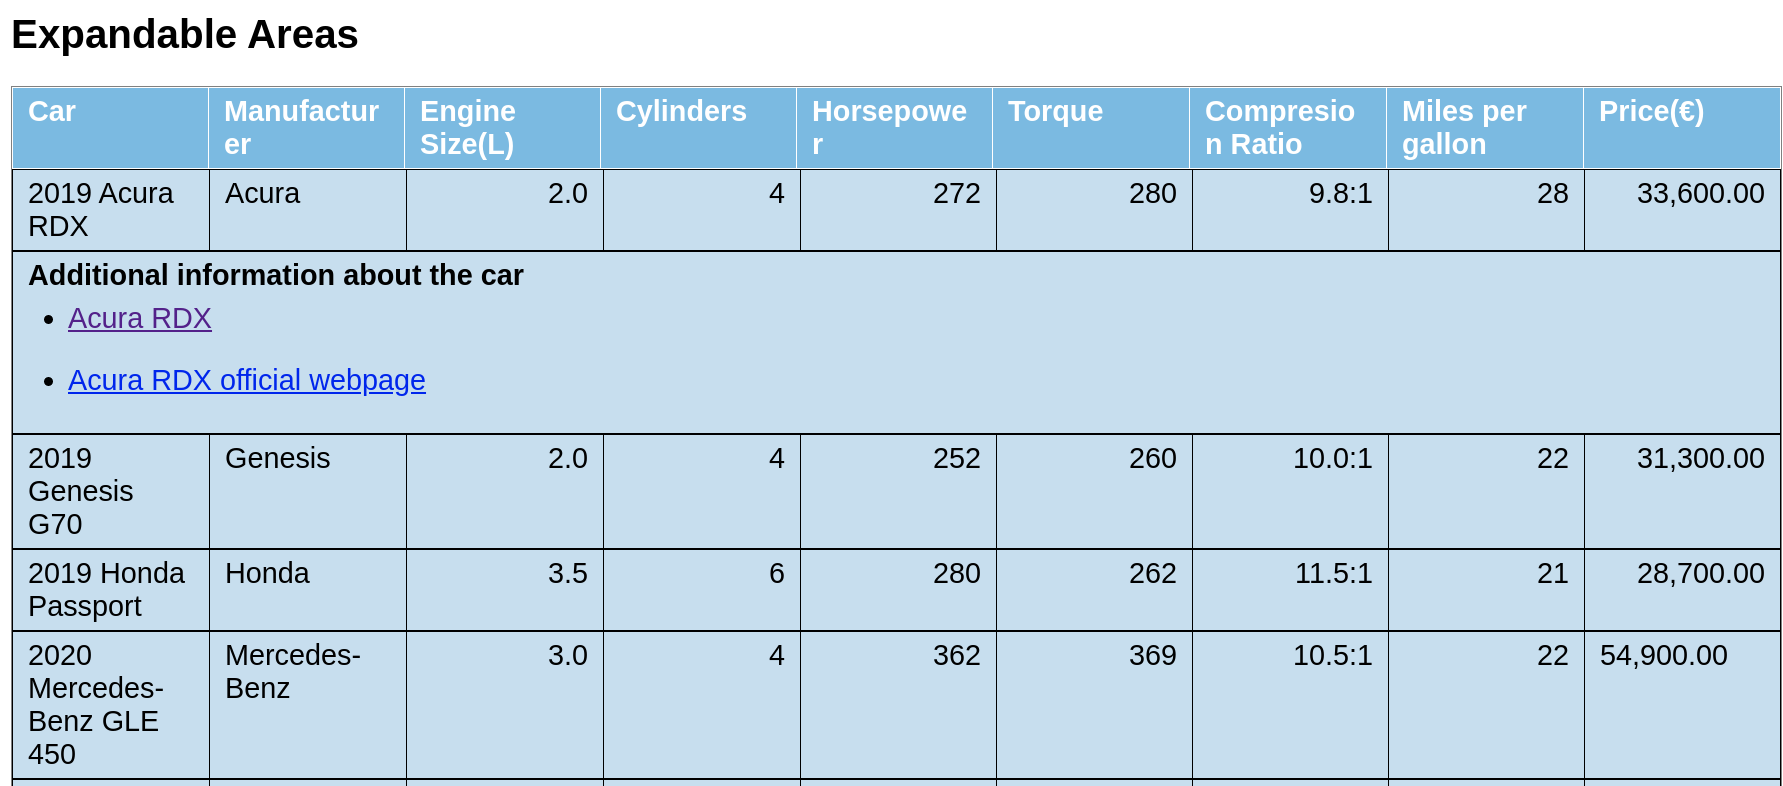
\includegraphics[width=\linewidth]
    {images/expandable_areas_after.png}%
    \label{alig1}%
    }


    \caption[Expandable Areas]
    {

    \imgcredit{Screenshot taken by the author.}
    }
    \label{figWhol}
\end{figure}

\section{Pagination (With Sort and Search)}
The amount of data increases every second, over 2.5 quintillion bytes of data are made every day and there is also estimation
 that in 2020 will be created 1.7MB of data in every second for each person in the world\parencite{PG_2}.
\newline
Tables are one of the best mediums for displaying large sets of data efficiently. Features can be added to tables to increase efficiency even more. For example, if a table is too long, it can be divided into `pages'. Each page houses a certain amount of rows. The user then can `flip' through these pages as page navigation is also implemented.

Furthermore, it is possible to sort the table by column (in ascending/descending and alphabetical order), and search for an element in the table.

This solution works for following browsers:
\begin{itemize}
    \item[--] Google Chrome
    \item[--] Mozzila Firefox
    \item[--] Internet Explorer
    \item[--] Opera
    \item[--] Microsoft Edge
\end{itemize}

For the implementation plug-in for the jQuery Javascript library called DataTables is used\parencite{PG_1}.


\begin{lstlisting}[%
    language = HTML,
    xleftmargin=0cm,              % no extra margins for floats
    xrightmargin=0cm,             % no extra margins for floats
    language=biblatex,
    basicstyle=\footnotesize\ttfamily,
    frame=shadowbox,
    numbers=left,
    label=list:BibACMIEEE,
     stringstyle=\color{blue}
    ,
]
    % An example of using Javascript plugin DataTable():
    %Include these two files in order to include additional advanced features to any HTML table
    %cdn.datatables.net/1.10.20/css/jquery.dataTables.min.css
    %cdn.datatables.net/1.10.20/js/jquery.dataTables.min.js

    $(document).ready(function(){
        $('#myTable').dataTable(); //this plugin provides searching, sorting and pagination
 });

\end{lstlisting}

Table is initilaized with "myTable" id and this id is used in
 ready function() to assign dataTable funcionality to our HTML table instance\parencite{PG}.

An example HTML table with this technique when using the sort feature on the \texttt{Price} column is shown below.
\begin{figure}[H]
    \centering

    {%
    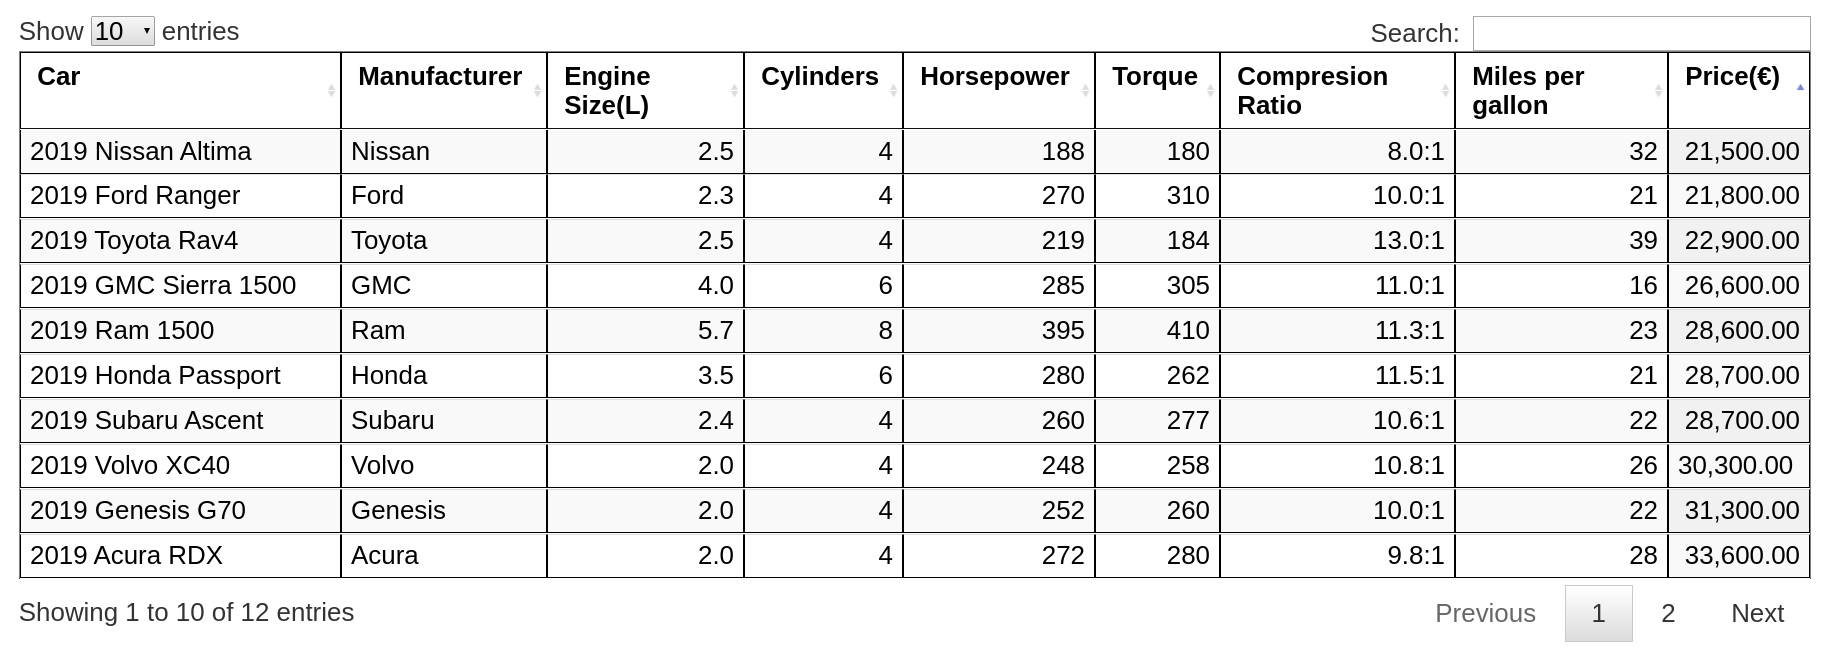
\includegraphics[width=\linewidth]
    {images/pagination_2.png}%
    \label{alig1}%
    }


    \caption[Pagination with sort option]
    {

    \imgcredit{Screenshot taken by the author.}
    }
    \label{figWhol}
\end{figure}

An example HTML table with this technique when using the search feature is shown below.
\begin{figure}[H]
    \centering

    {%
    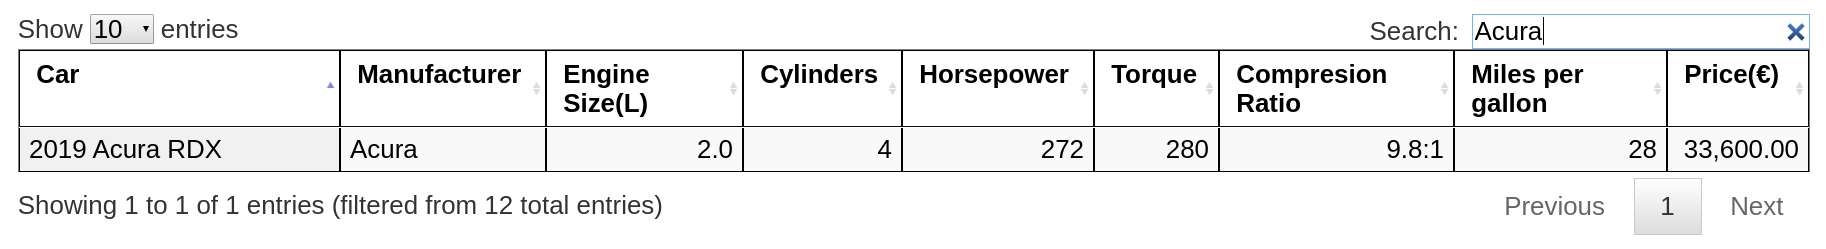
\includegraphics[width=\linewidth]
    {images/pagination_1.png}%
    \label{alig1}%
    }


    \caption[Pagination with search option]
    {

    \imgcredit{Screenshot taken by the author.}
    }
    \label{figWhol}
\end{figure}

\newpage

\chapter{Responsive Tables}

Due to the increasing amount of screens and their varying shapes, sizes,
and developers' space allocation when designing and implementing tables,
responsive table techniques have been `developed' by manipulating the table's
columns and rows to provide an optimal experience for users across most mediums. It means the row and
columns can be repositioned,
resized, collapsed, minimized, etc..

Data tables can contain many information, which makes displaying that data quite messy and hard to
look at. So by using responsive design, a big favor is done to the clients,
by adjusting the table according to their devices. One idea would be to minimize the table, but if the user is looking
at the table from his mobile device, he would have to zoom in, which is not that useful to him, because then again he would need to scroll
to view the whole table \parencite{9}.

\begin{figure}[H]
    \centering

    {%
    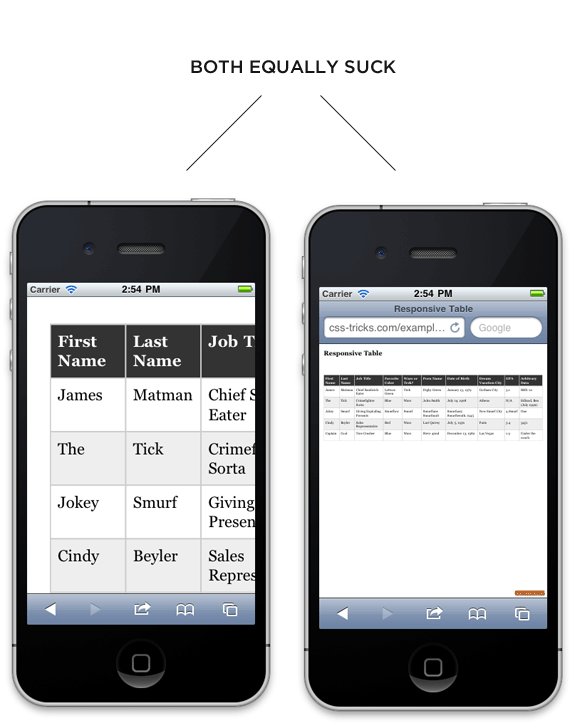
\includegraphics[width=\linewidth]
    {images/zoom_1.png}%
    \label{alig1}%
    }


    \caption[Before reponsive]
    {

    \imgcredit{https://css-tricks.com/responsive-data-tables/.}
    }
    \label{figWhol}
\end{figure}

As seen in the figure above, both options do not really look nor perform well.
So, by using some simple CSS it is possible to fix that problem. With the help of the mentioned
media queries, it is possible to specify for which device sizes, which settings should be used.

\begin{lstlisting}[%
    language = HTML,
    xleftmargin=0cm,              % no extra margins for floats
    xrightmargin=0cm,             % no extra margins for floats
    language=biblatex,
    basicstyle=\footnotesize\ttfamily,
    frame=shadowbox,
    numbers=left,
    label=list:BibACMIEEE,
     stringstyle=\color{blue}
    ,
]
    % An example of using simple CSS with media queries on how to achieve Responsive Design:

    @media
only screen and (max-width: 760px),
(min-device-width: 768px) and (max-device-width: 1024px)  {

	/* Force table to not be like tables anymore */
	table, thead, tbody, th, td, tr {
		display: block;
	}

	/* Hide table headers (but not display: none;, for accessibility) */
	thead tr {
		position: absolute;
		top: -624.9375rem;
		left: -624.9375rem;
	}

	tr { border: 1px solid #ccc; }

	td {
		/* Behave  like a "row" */
		border: none;
		border-bottom: 1px solid #eee;
		position: relative;
		padding-left: 50%;
	}

	td:before {
		/* Now like a table header */
		position: absolute;
		/* Top/left values mimic padding */
		top: 0;
		left: 0.375rem;
		width: 45%;
		padding-right: 0.625rem;
		white-space: nowrap;
	}

\end{lstlisting}

And now, the end result is seen in the image below.
\begin{figure}[H]
    \centering

    {%
    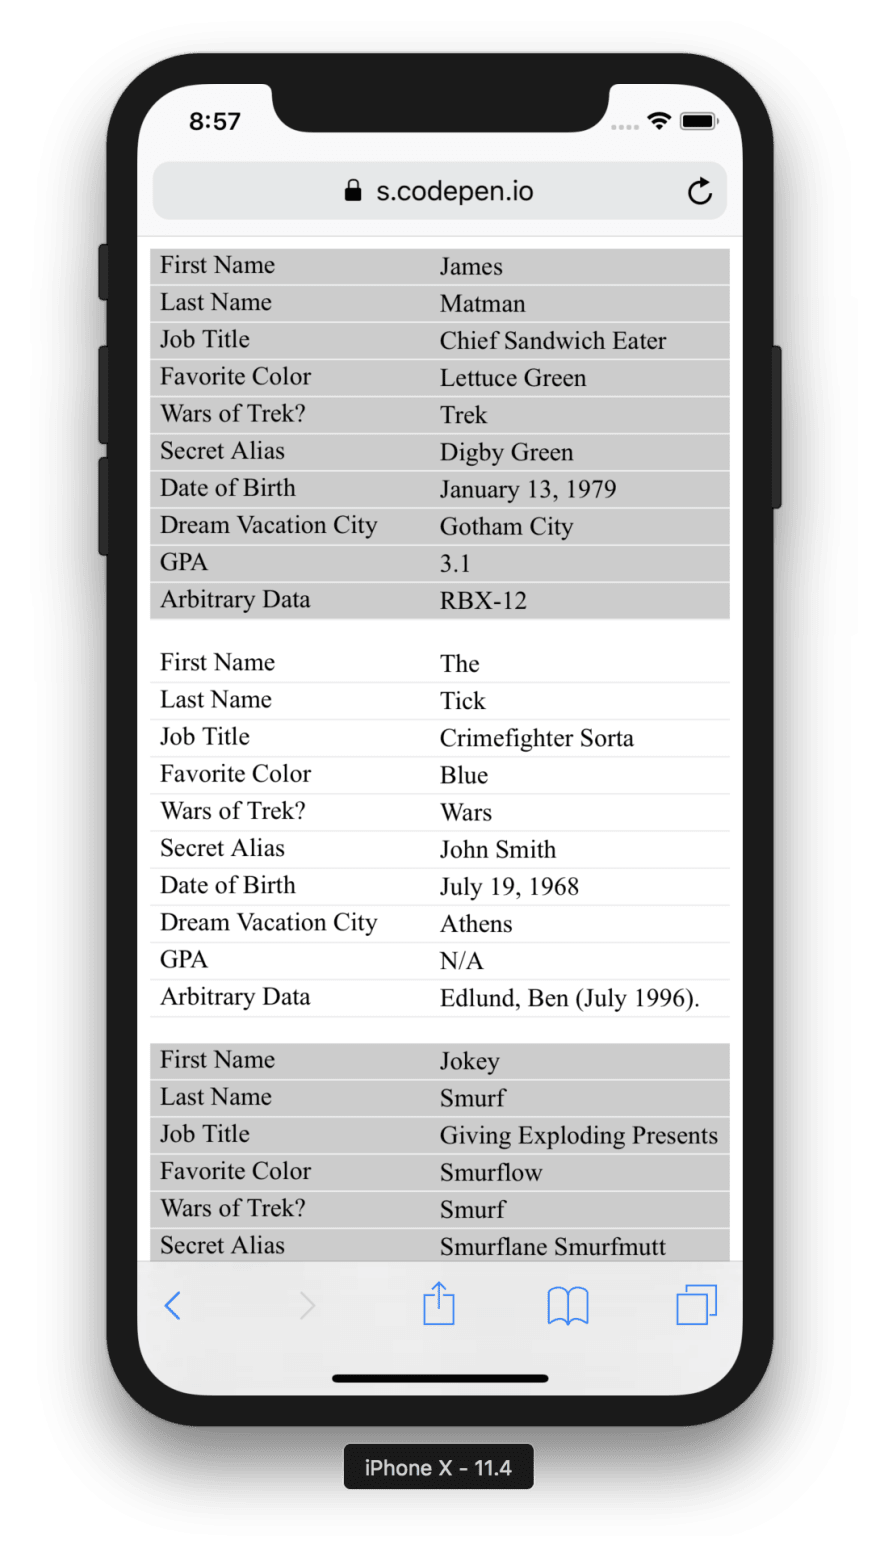
\includegraphics[width=0.45\linewidth]
    {images/zoom_3.png}%
    \label{alig1}%
    }


    \caption[After reposnsive]
    {

    \imgcredit{https://css-tricks.com/responsive-data-tables/.}
    }
    \label{figZoom3}
\end{figure}


Some of the most popular techniques are:
\begin{itemize}
    \item[--] Hidden Columns - Selected by User
    \item[--] Horizontal Scroll
    \item[--] Fixed Header
    \item[--] Flip Scroll
    \item[--] User Resizeable Columns
    \item[--] Long Two Column
\end{itemize}

In the following sections we will try to give a brief but detailed description of what exactly each technique consists of, as well as the reason to include this techniques on tables, and the code required to implement such techniques.

\newpage
\section{Horizontal Scroll}
When the allocated space is too small - horizontally, instead of hiding it, a horizontal scroll bar (just for the table) is created. The user can then scroll away.

Horizontal Scrolling represents a technique that resizes the table
into columns at small screen resoultion \parencite{HS_1}. 
This is different from viewport scrolling as we scroll only through the table.

It is very useful technique when presenting large data
 sets with identifiers in the first column. Then is very easy for every user to compare data content with multiple identifiers\parencite{HS}.

This solution works for following browsers:
\begin{itemize}
    \item[--] Google Chrome
    \item[--] Mozzila Firefox
    \item[--] Internet Explorer
    \item[--] Opera
    \item[--] Microsoft Edge
\end{itemize}

It is impossible to find one size that fits all solution. Data comparing is very difficult on the small screens.
There are a lot of possible workarounds for this issue, but no one can solve this problem \parencite{HS_1}.
Our implementation of horizontal scrolling creates table elements scrollable, but also can not solve the issue to the end\parencite{HS_1}.

The code required to implement this technique on a table is shown below.

\begin{lstlisting}[%
    language = HTML,
    xleftmargin=0cm,              % no extra margins for floats
    xrightmargin=0cm,             % no extra margins for floats
    language=biblatex,
    basicstyle=\footnotesize\ttfamily,
    frame=shadowbox,
    numbers=left,
    label=list:BibACMIEEE,
     stringstyle=\color{blue}
    ,
]
.rtable {

    display: inline-block;
    vertical-align: top;
    max-width: 100%;

    overflow-x: auto;

    // optional - looks better for small cell values
    white-space: nowrap;

    border-collapse: collapse;
    border-spacing: 0;
}

\end{lstlisting}

This CSS code represents CSS class \texttt{.rtable} used in the case when container is not resized.
With display: inline-block all items are listed horizontally instead of vertically.

\texttt{vertical-align} property maintains how elements set next to each other in a line.

The \texttt{overflow} property determines whether to crop content or to add scroll bars (along the x-axis) when a table's content is too big to satisfy some screen resolution.

We can use \texttt{white-space: nowrap} property as optional for small cell values.
Css border properties are used to control borders into a table\parencite{HS_1}.

An example HTML table with this technique is shown below.
\begin{figure}[H]
    \centering

    {%
    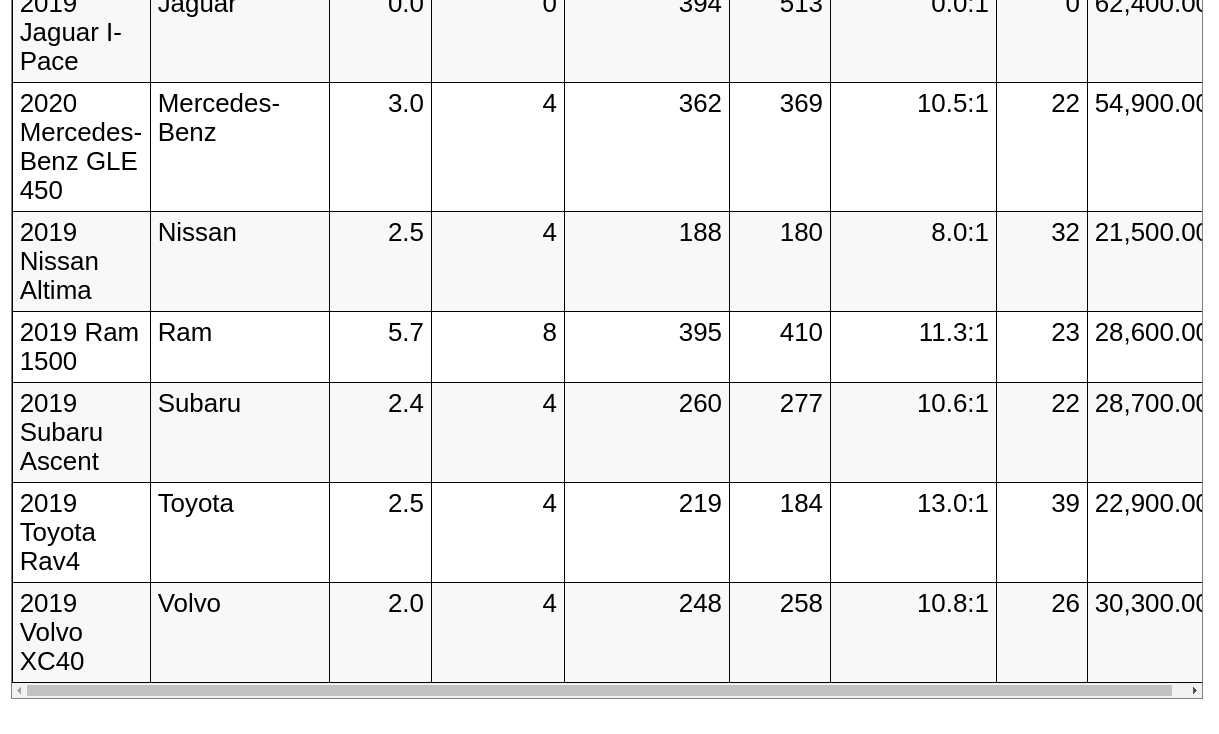
\includegraphics[width=1\linewidth]
    {images/horizontal.png}%
    \label{alig1}%
    }


    \caption[Horizontal Scroll]
    {

    \imgcredit{Screenshot taken by the author.}
    }
    \label{figWhol}
\end{figure}

\newpage
\section{Fixed Header}
When the table is vertically long, the table's header is fixed to the top of the table's view.
As we scroll down, the table's header is kept always visible.

It is very useful to have the fixed header (first row containing the header cells) fixed on the top of the table, when presenting tables with a particularly larage data set. This helps users to quickly determine what every column identify rather than need to scroll back to the top of the table every time.

Fixed Header provides information that allows the user to always know in what column the cell the user is looking at is in.

This is very effective feature that makes our life easier \parencite{HS}.

This solution works for following browsers:
\begin{itemize}
    \item[--] Google Chrome
    \item[--] Mozzila Firefox
    \item[--] Internet Explorer
    \item[--] Opera
    \item[--] Microsoft Edge
\end{itemize}

\begin{lstlisting}[%
    language = HTML,
    xleftmargin=0cm,              % no extra margins for floats
    xrightmargin=0cm,             % no extra margins for floats
    language=biblatex,
    basicstyle=\footnotesize\ttfamily,
    frame=shadowbox,
    numbers=left,
    label=list:BibACMIEEE,
     stringstyle=\color{blue}
    ,
]
.fixedHeader tbody {
    display: block;
    overflow: auto;
    width: 100%;
}

.fixedHeader thead tr {
    display: table;
    width: 100%;
    table-layout: fixed;
}

.fixedHeader thead, .fixedHeader tbody tr {
    display: table;
    width: 100%;
    table-layout: fixed;
}

.fixedHeader thead {
    width: calc( 100% - 0.6em )
}

.fixedHeader td {
    width: 100%;
}

\end{lstlisting}

$<$\texttt{tbody}$>$ element is determined with the type of rendering box.

With \texttt{overflow: auto}, a scrollbar will appear along y-axis.

All $<$\texttt{thead}$>$ and $<$\texttt{tbody}$>$ rows will behave as table elements.

Fixed table layout algorithm is used to control table and column widths.

Width for almost every table element is static, just the header has non-static width \parencite{FH_1}.

The width of header is determined with the \texttt{calc()} function to allow responsiveness \parencite{FH}.

An example HTML table with this technique is shown below.

\begin{figure}[H]
    \centering

    {%
    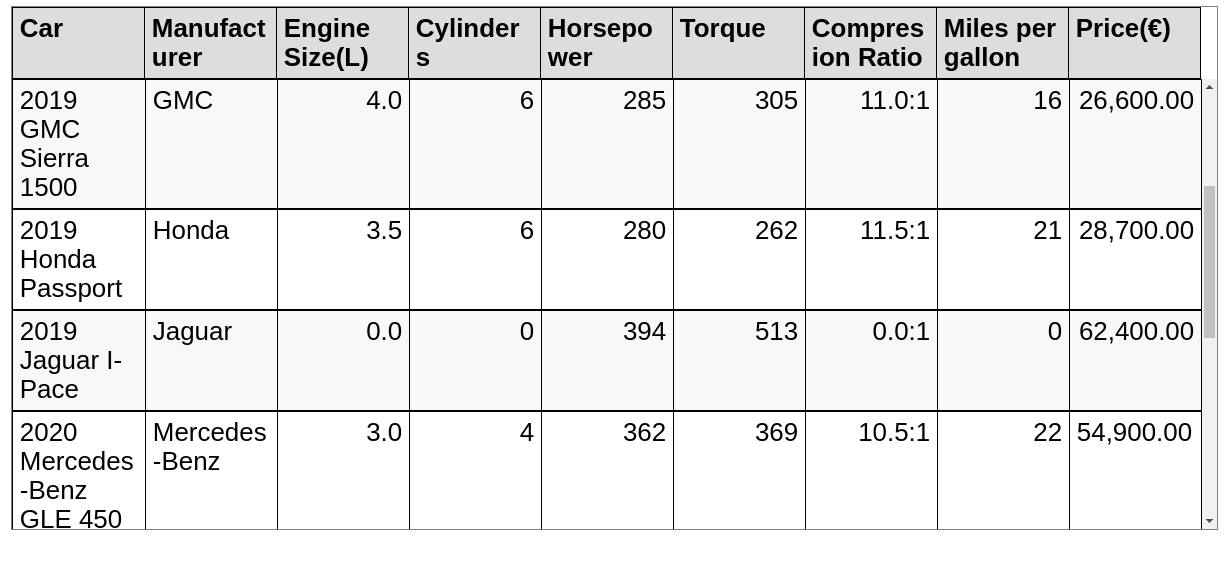
\includegraphics[width=1\linewidth]
    {images/fixed_header.png}%
    \label{alig1}%
    }


    \caption[Fixed Header]
    {

    \imgcredit{Screenshot taken by the author.}
    }
    \label{figWhol}
\end{figure}


\newpage
\section{Flip Scroll}
This technique is useful for an object-based table; one where each row is populated by a single `object' where each column represents a different feature of the object. If all features -- columns -- cannot be seen at once, it is sometimes more desireable to be able to show all features of an object rather than a good amount of (incomplete) features for a good amount of objects.
\newline

Rather than having the user scroll through features, the user is now able to scroll through objects horizontally instead. This is the result of transposing the table. The first column will now house the (previously column) headers and each column will be devoted to an object, rather than each row.

Flip scroll also `promises' to keep the table in the allocated space -- by allowing table horizontal scrolling.

This solution works for following browsers:
\begin{itemize}
    \item[--] Google Chrome
    \item[--] Mozzila Firefox
    \item[--] Internet Explorer
    \item[--] Opera
    \item[--] Microsoft Edge
\end{itemize}

\begin{lstlisting}[%
    language = CSS,
    xleftmargin=0cm,              % no extra margins for floats
    xrightmargin=0cm,             % no extra margins for floats
    language=biblatex,
    basicstyle=\footnotesize\ttfamily,
    frame=shadowbox,
    numbers=left,
    label=list:BibACMIEEE,
     stringstyle=\color{blue}
    ,
]
table.flipscroll{
    width: 100%;
    overflow-x: auto;
}
  
table.flipscroll  tbody tr { 
    display: inline-block; 
    vertical-align: top; 
}
  
table.flipscroll  tbody { 
    display: block; 
    width: auto; 
    position: relative; 
    overflow-x: auto; 
    white-space: nowrap; 
}

\end{lstlisting}

Setting \texttt{width: 100\%} and \texttt{overflow-x: auto} makes the table horizontally scrollable and stick to the allocated space.

The trick is setting the attribute \texttt{display: inline-block} on the \texttt{tbody tr} HTML tag and \texttt{white-space: nowrap} on the \texttt{tbody} HTML tag \parencite{FS}.

Following image represents an HTML table with Flip Scroll:

\begin{figure}[H]
    \centering

    {%
    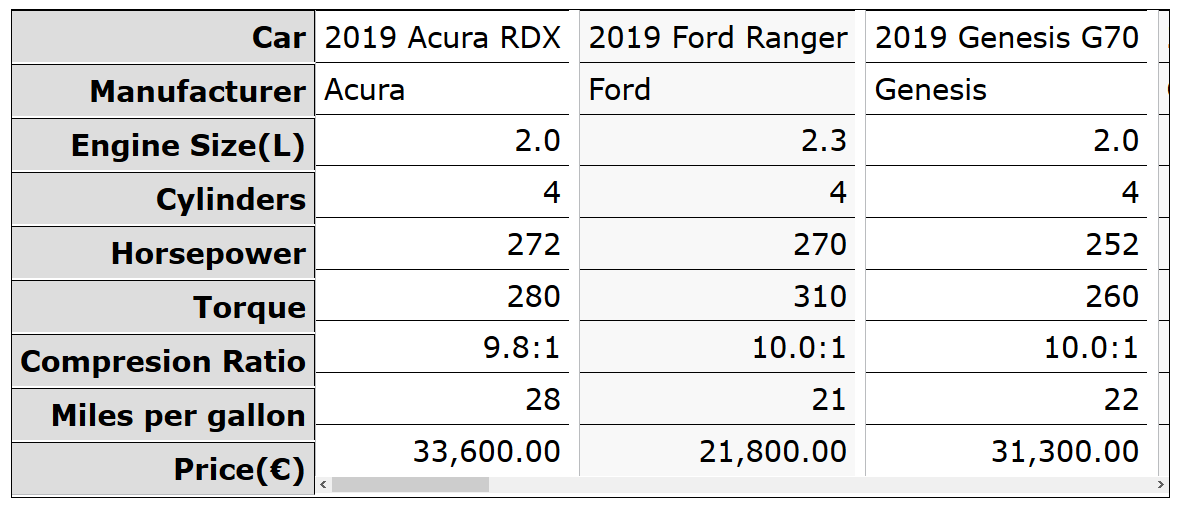
\includegraphics[width=1\linewidth]
    {images/flip_scroll.png}%
    \label{alig1}%
    }


    \caption[Flip Scroll]
    {

    \imgcredit{Screenshot taken by the author.}
    }
    \label{figFlipScroll}
\end{figure}


\newpage
\section{User Resizeable Columns}
This technique empowers the user quite significantly. As the title suggests, the user is able to manipulate the size of a table's columns. 

This technique is useful when the user is immune to space limitation penalties the table might have on most other users. For example, if a user has a screen big enough that space between columns is wasted to keep column sizes consistent, being able to resize this column to bring other columns into view is highly desireable.

User Resizeable Columns allows the user to tailor the table's experience to his/her own preferences. 

There are two possible solutions. Both work for following browsers:
\begin{itemize}
    \item[--] Google Chrome
    \item[--] Mozzila Firefox
    \item[--] Internet Explorer
    \item[--] Opera
    \item[--] Microsoft Edge
\end{itemize}

Solution using only CSS and HTML:
\begin{lstlisting}[%
    language = HTML,
    xleftmargin=0cm,              % no extra margins for floats
    xrightmargin=0cm,             % no extra margins for floats
    language=biblatex,
    basicstyle=\footnotesize\ttfamily,
    frame=shadowbox,
    numbers=left,
    label=list:BibACMIEEE,
     stringstyle=\color{blue}
    ,
]
<thead>
    <tr>
        <th title="Car">
            <div class = "resizecell">Car</div>
        </th>
        <th title="Manufacturer">
            <div class = "resizecell">Manufacturer</div>
        </th>
        <th title="Engine Size(L)">
            <div class = "resizecell">Engine Size(L)</div>
        </th>
        [...]
    </tr>
</thead>
\end{lstlisting}

\begin{lstlisting}[%
    language = CSS,
    xleftmargin=0cm,              % no extra margins for floats
    xrightmargin=0cm,             % no extra margins for floats
    language=biblatex,
    basicstyle=\footnotesize\ttfamily,
    frame=shadowbox,
    numbers=left,
    label=list:BibACMIEEE,
     stringstyle=\color{blue}
    ,
]
.resizecell {
    resize: horizontal;
    overflow: auto;
    width: 100%;
    hyphens: auto;
}
\end{lstlisting}

Encapsulating every header cell (or every single cell) with a \texttt{$<$div$>$} tag allows CSS to enable resizeability by setting the attribute \texttt{resize: horizontal} to these divs \parencite{URC_1}.

Following image represents an HTML table with User Resizeable Columns using only HTML and CSS:

\begin{figure}[H]
    \centering

    {%
    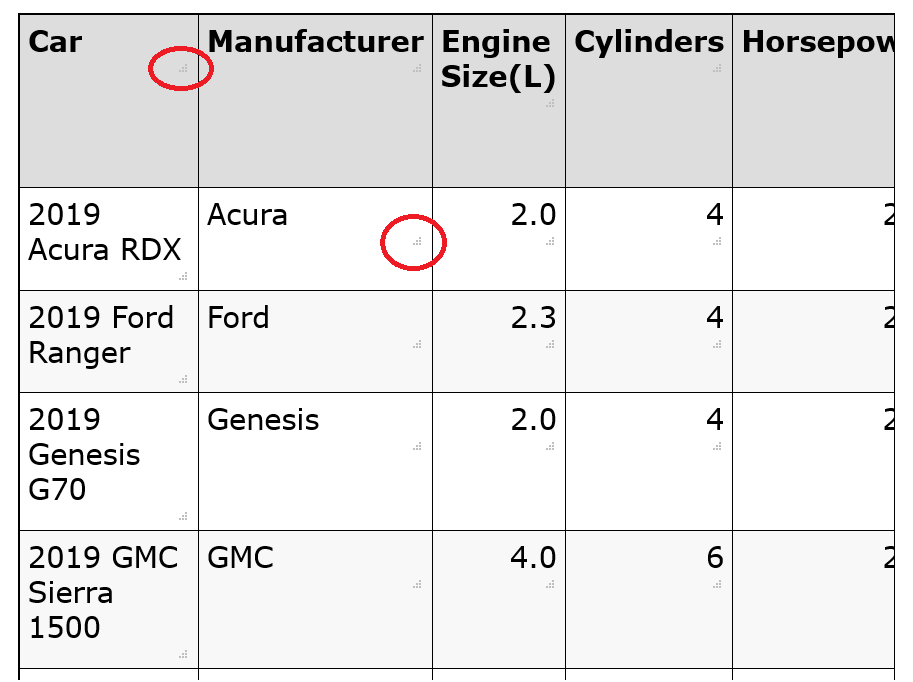
\includegraphics[width=1\linewidth]
    {images/urc_css.png}%
    \label{alig1}%
    }


    \caption[User Resizeable Columns using only HTML and CSS]
    {

    \imgcredit{Screenshot taken by the author.}
    }
    \label{figURCCSS}
\end{figure}

Solution using JavaScript (jQuery):
\begin{lstlisting}[%
%    language = JavaScript,
    xleftmargin=0cm,              % no extra margins for floats
    xrightmargin=0cm,             % no extra margins for floats
    language=biblatex,
    basicstyle=\footnotesize\ttfamily,
    frame=shadowbox,
    numbers=left,
    label=list:BibACMIEEE,
     stringstyle=\color{blue}
    ,
]
~/js/jQuery.resizableColumns.js

$(function(){
  $('.rcl').resizeableColumns();
});
\end{lstlisting}

The trick is calling the \texttt{resizeableColumns()} on the table of your choice \parencite{URC_2}.

\begin{figure}[H]
    \centering

    {%
    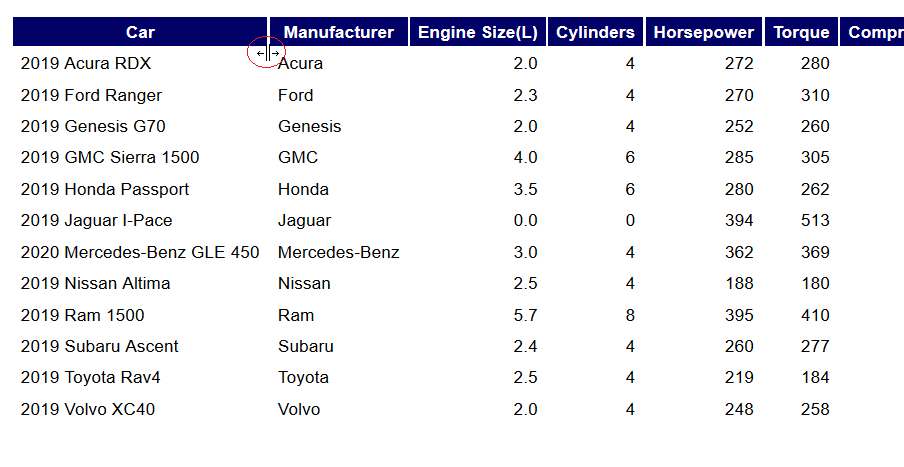
\includegraphics[width=1\linewidth]
    {images/urc_js.png}%
    \label{alig1}%
    }


    \caption[User Resizeable Columns using JS (jQuery)]
    {

    \imgcredit{Screenshot taken by the author.}
    }
    \label{figURCJS}
\end{figure}

\newpage
\section{Long Two Column}
Just like Flip Scroll, this technique is useful for an object-based table; one where each row is populated by a single `object' where each column represents a different feature of the object. 
\newline

Rather than having the user scroll through features, the user is now able to scroll through objects vertically instead. This is the result of transposing the table. The first column will now house the (previously column) headers and the second column will house the data previously housed in the first row. This creates a `minitable' for the (previously) first row. For the next object (and row), another `minitable' is created like with the first one and then appended below. This approach creates a `minitable' for each object and appends it to the previous object. 

As the name suggest, you end up with a long table of 2 columns, the first of which is 'always the same'.

Unlike Flip scroll, it does not keep the table in the allocated space, unless you set vertical scrolling.

This solution works for following browsers:\begin{itemize}
    \item[--] Google Chrome
    \item[--] Mozzila Firefox
    \item[--] Internet Explorer
    \item[--] Opera
    \item[--] Microsoft Edge
\end{itemize}

\begin{lstlisting}[%
    language = CSS,
    xleftmargin=0cm,              % no extra margins for floats
    xrightmargin=0cm,             % no extra margins for floats
    language=biblatex,
    basicstyle=\footnotesize\ttfamily,
    frame=shadowbox,
    numbers=left,
    label=list:BibACMIEEE,
     stringstyle=\color{blue}
    ,
]
table, thead, tbody, th, td, tr {
    display: block;
}

td {
    /* Behave  like a "row" */
    border: none;
    border-bottom: 1px solid #eee;
    position: relative;
    padding-left: 50%;
}

td:before {
    /* Now like a table header */
    position: absolute;
    /* Top/left values mimic padding */
    top: 0;
    left: 6px;
    width: 45%;
    padding-right: 0.625rem;
    white-space: nowrap;
}
\end{lstlisting}

The trick is setting the table's elements to \texttt{display: block} and the $<$\texttt{td}$>$ tag's attribute to \texttt{position: relative} \parencite{L2C}.

Following image represents an HTML table with Long Two Column:

\begin{figure}[H]
    \centering

    {%
    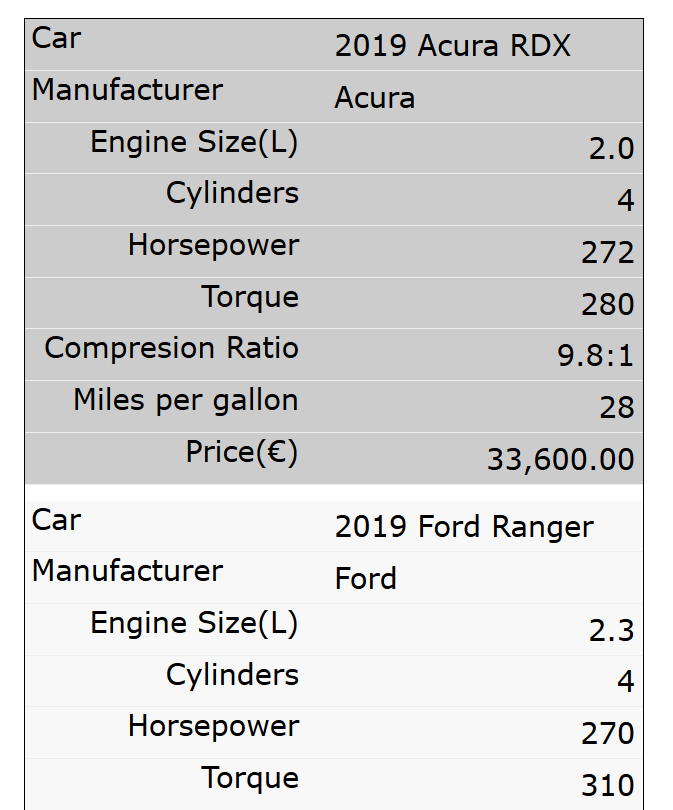
\includegraphics[width=1\linewidth]
    {images/long_two_column.png}%
    \label{alig1}%
    }


    \caption[Long Two Column]
    {

    \imgcredit{Screenshot taken by the author.}
    }
    \label{figLongTwoColumn}
\end{figure}
